\documentclass{beamer}

\usepackage[utf8]{inputenc}
\usepackage{epstopdf}
\usepackage{textpos}
\usepackage{textcomp}
\usepackage{verbatim}
\usepackage{varwidth}
\usepackage{amsmath}
\usepackage{amsfonts}
\usepackage{algorithmic}
\usepackage[linesnumbered,ruled]{algorithm2e}
\usepackage{graphicx}
%\usepackage{lipsum}
%\usepackage{dblfloatfix}
%\usepackage{multicol}
%\usepackage[ruled]{algorithm2e}

\usefonttheme[onlymath]{serif}
%\setlength{\columnsep}{5cm}

\setbeamertemplate{caption}[numbered]

% standard, good-looking theme
\usetheme{Madrid}

% this should put the outline on the header of each page
% can't make it look right, though
% \usetheme{Darmstadt}

\title[Capstone]{An optimization-inspired approach to parallel sorting}

\author{Team Metropolis:\\
James Farzi, JJ Lay, Graham West}
%\date{COMS Seminar}%, August 2016}
\date{February 13, 2019}

%\institute
%{
%	GTA, Computational Science\\
%	Middle Tennessee State University\\
%	Research Advisor: John Wallin\\
%}

%%%%%%%%% BEGIN DOCUMENT %%%%%%%%%
%%%%%%%%% BEGIN DOCUMENT %%%%%%%%%
%%%%%%%%% BEGIN DOCUMENT %%%%%%%%%

\begin{document}

% get title page 
\frame{\titlepage}

\begin{frame}	
	\frametitle{Outline}
	\tableofcontents	
\end{frame}

%%%%%%%%%%%%%
%%%%%%%%%%%%%
\section{The Algorithm}

\begin{frame}	
	\begin{Huge}
		\begin{center}
			The Algorithm
		\end{center}
	\end{Huge}
\end{frame}

\begin{frame}	
	\frametitle{The Algorithm}
	
	\begin{block}{xxx}
		\begin{itemize}
			\item xxx
			\item xxx
		\end{itemize}
	\end{block}
	
	\begin{block}{xxx}
		\begin{itemize}
			\item xxx
			\item xxx
		\end{itemize}
	\end{block}
\end{frame}

\subsection{Distributing/Importing Files}

\begin{frame}	
	\frametitle{Distributing/Importing Files}
	
	\begin{block}{xxx}
		\begin{itemize}
			\item xxx
			\item xxx
		\end{itemize}
	\end{block}
	
	\begin{block}{xxx}
		\begin{itemize}
			\item xxx
			\item xxx
		\end{itemize}
	\end{block}
\end{frame}

\subsection{Sorting}

\begin{frame}	
	\frametitle{Sorting}
	
	We implemented Merge and Bubble Sort
	
	\begin{block}{xxx}
		\begin{itemize}
			\item xxx
			\item xxx
		\end{itemize}
	\end{block}
	
	\begin{block}{xxx}
		\begin{itemize}
			\item xxx
			\item xxx
		\end{itemize}
	\end{block}
\end{frame}

\subsection{Binning}

\begin{frame}	
	\frametitle{Binning}
	
	\begin{block}{Binary search}
		\begin{itemize}
			\item Since the data is sorted, we can use a binary search to find where the bin edges lie in index space
			\item We can then subtract successive edges' indices to find the number of elements in that bin
		\end{itemize}
	\end{block}
	
	\begin{block}{xxx}
		\begin{itemize}
			\item xxx
			\item xxx
		\end{itemize}
	\end{block}
\end{frame}

\begin{frame}
	\frametitle{Binning}
	
	\begin{block}{Adapting the bins}
		for interior bin edges (endpoint bins stay constant):
		\begin{equation}
			\begin{split}
				\Delta C & = 2.0 ( c_i^n - c_{i-1}^n ) / ( c_i^n + c_{i-1}^n ) \\
				\Delta B & = b_{i+1}^n - b_i^n \\
				b_i^{n+1} & = b_i^n + \alpha \Delta C \Delta B
			\end{split}
		\end{equation}
		where $0 < \alpha < 0.5$ and $b_i^n < b_{i+1}^n$ for all $n$
	\end{block}
	
	\begin{block}{Uniformity metric}
		\begin{equation}
			U^n = \textrm{max}( \dfrac{c_{\textrm{max}} - c_{\textrm{avg}}}{c_{\textrm{avg}}}, \dfrac{c_{\textrm{avg}} - c_{\textrm{min}}}{c_{\textrm{avg}}} )
		\end{equation}
	\end{block}
\end{frame}

\begin{frame}
	\frametitle{Binning}
	
	\begin{figure}[!htb]
		\centering
		\vspace{-5pt}
		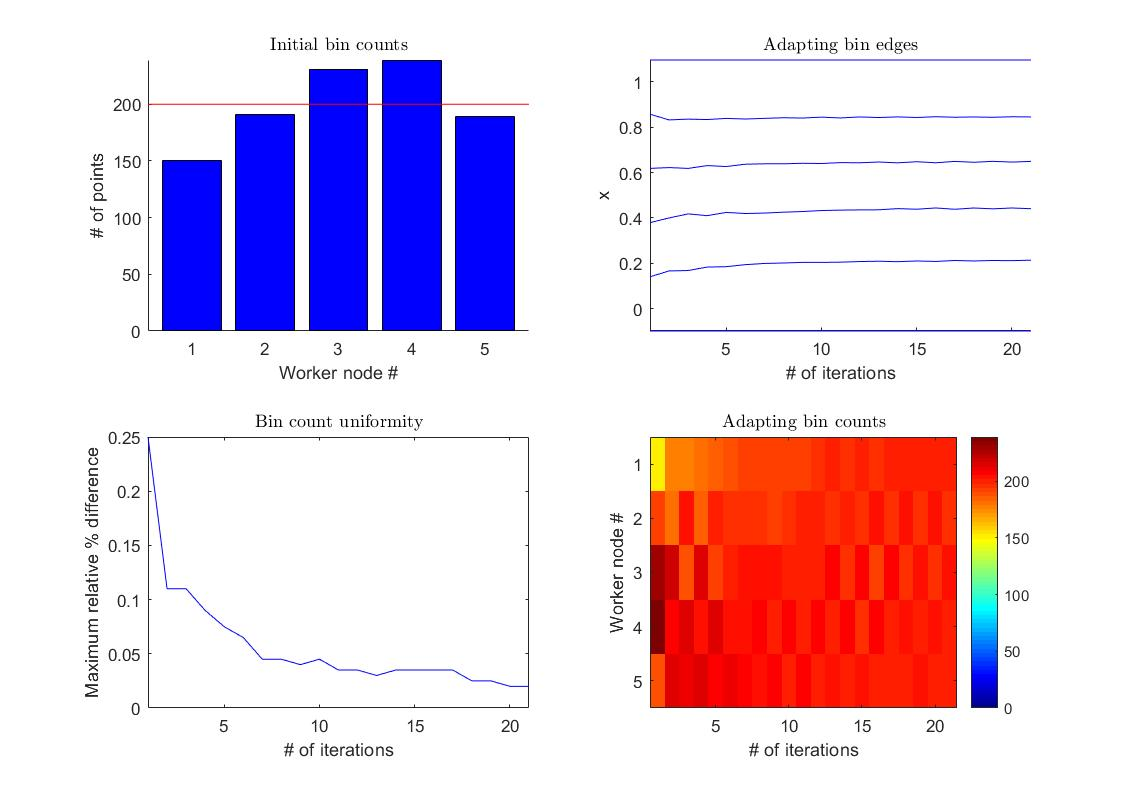
\includegraphics[scale = 0.25]{AdaptiveBinning_5Nodes_1000Lines_AverageLine}
		\vspace{-10pt}
		\caption{Using 5 nodes to uniformly bin 1000 data points}
	\end{figure}
\end{frame}

\subsection{Exchanging data}

\begin{frame}	
	\frametitle{Exchanging data}
	
	\begin{block}{xxx}
		\begin{itemize}
			\item xxx
			\item xxx
		\end{itemize}
	\end{block}
	
	\begin{block}{xxx}
		\begin{itemize}
			\item xxx
			\item xxx
		\end{itemize}
	\end{block}
\end{frame}


%%%%%%%%%%%%
%%% new section %%%
%%%%%%%%%%%%
\section{Testing}

\begin{frame}	
	\begin{Huge}
		\begin{center}
			Testing
		\end{center}
	\end{Huge}
\end{frame}

\subsection{Methodology}


\subsection{Results}

%%%%%%%%%%%%
%%% new section %%%
%%%%%%%%%%%%
\section{Conclusions}

\begin{frame}	
	\begin{Huge}
		\begin{center}
			Conclusions
		\end{center}
	\end{Huge}
\end{frame}



%%%%%%%%%%%%%%%%%%%%%%%
%%%%%%%%%%%%%%%%%%%%%%%
%% Leftover for reference and copying code %%
%%%%%%%%%%%%%%%%%%%%%%%
%%%%%%%%%%%%%%%%%%%%%%%


\begin{frame}
	\frametitle{RSAP}
	
	\begin{block}{1D proposal}
		RSAP proposal-scaling
		\vspace{-15pt}
		
		\begin{equation}
			\begin{split}
				A_{t}(k_t^n) & = 1 - (1- \hat A_t)(1-\textrm{exp}(-r_t k_t^n))\\
				A_{w}(k_w^n) & = 1 - (1- \hat A_w)(1-\textrm{exp}(-r_w k_w^n))
			\end{split}
		\end{equation}
		where $r_{w}>0$, $r_{t}>0$, $\hat A_{w}>1$, $0<\hat A_{t}<1$
		
		\vspace{5pt}
		Properties
		\begin{itemize}
			\item $k_t^n, k_w^n$ are counters
			\item Initial/reset value is 0 ($\sigma_{t} = \sigma_{w} = \sigma_{f}$)
			\item Asymptotic: $A_t, A_w \rightarrow \hat A_t, \hat A_w$ as $k \rightarrow \infty$
		\end{itemize}
%		\vspace{5pt}
		
%		Optimal values: $ r_t, r_w = 0.3, A_t = 0.1, A_w = 10$
	\end{block}
\end{frame}

\begin{frame}
	\frametitle{RSAP}
	
	\begin{block}{1D proposal}
		RSAP proposal-scaling
		\vspace{-15pt}
		
		\begin{equation}
			\begin{split}
				A_{t}(k_t^n) & = 1 - (1- \hat A_t)(1-\textrm{exp}(-r_t k_t^n))\\
				A_{w}(k_w^n) & = 1 - (1- \hat A_w)(1-\textrm{exp}(-r_w k_w^n))
			\end{split}
		\end{equation}
		where $r_{w}>0$, $r_{t}>0$, $\hat A_{w}>1$, $0<\hat A_{t}<1$
		
		\vspace{5pt}
		Rules
		\begin{itemize}
			\item If a candidate is \textbf{rejected}, \textbf{increment} the counter of the proposal used (thin/wide)
			\item If a candidate is \textbf{accepted}, \textbf{reset} all counters
			\item At each step, set $\sigma_t^n = \sigma_f A_{t}(k_t^n)$, $\sigma_w^n = \sigma_f A_{w}(k_w^n)$ \\
		\end{itemize}
	\end{block}
\end{frame}

\begin{frame}
	\frametitle{Introduction to MCMC}
	
	\begin{figure}[!htb]
		\centering
		\includegraphics[scale = 0.25]{MCMC_Illust_05}
	\end{figure}
	Candidate state $\theta' = 1.76$ accepted \\ % definitely accepted
	Chain: $2.0, 2.0, 1.76$
\end{frame}

\begin{frame}	
	\frametitle{Introduction to MCMC}
	
	\begin{figure}[!htb]
		\centering

		\minipage{0.5\textwidth}
			\includegraphics[scale = 0.09]{PosterPlot_Ackley_Function_thin_00}
		\endminipage\hfill %%%%%%%%%%%%%%%%%%%
		\minipage{0.5\textwidth}
			\includegraphics[scale = 0.09]{PosterPlot_Ackley_Chain_thin_00}
		\endminipage\hfill
		\minipage{0.4\textwidth}
			\includegraphics[scale = 0.075]{PosterPlot_Ackley_Dist_thin_00}
		\endminipage\hfill
		\minipage{0.6\textwidth}
			\caption{Metropolis run over a 1D Ackley function with a proposal width of $\sigma = 0.35$.}
			\vspace{-10pt}
			\begin{equation}
				\begin{split}
					\hspace{ -30pt} f(\theta) = & \hspace{3pt} a \Big( 1 - \textrm{exp}(- 0.2 |\theta|) \Big) + \\
									& \hspace{4pt} b \Big( e - \textrm{exp}(\textrm{cos}(2 \pi \theta)) \Big)
				\end{split}
			\end{equation}
		\endminipage\hfill
	\end{figure}
	
	% all the garbage in the distribution plot is the burn-in
	
\end{frame}

\begin{frame}	
	\frametitle{Introduction to MCMC}
	
	\begin{algorithm}[H]
	\begin{algorithmic}[1]
		\STATE Initialize $\theta^0$
		\FOR{ $n = 1$ \TO $N$}
			\STATE Generate $\theta' \sim q(\theta'|\theta^{n-1})$
			\STATE \begin{varwidth}[t]{\linewidth}
			Compute $\alpha(\theta'|\theta^{n-1}) = \textrm{min}\Bigg(1, \dfrac{\pi(\theta'|y)} {\pi(\theta^{n-1}|y)}\Bigg)$ \par
			\hskip\algorithmicindent \hspace{1.137in} $=\textrm{min}\Bigg(1, \dfrac{\ell(y|\theta')p(\theta')} {\ell(y|\theta^{n-1})p(\theta^{n-1})}\Bigg)$
			\end{varwidth}
			\STATE Set $\theta^n = \theta'$ with probability $\alpha$, else $\theta^n = \theta^{n-1}$
		\ENDFOR
	\end{algorithmic}
	\caption{The Metropolis method}
	\end{algorithm}
	
\end{frame}

\begin{frame}	
	\frametitle{Introduction to MCMC}
	
	\begin{figure}[!htb]
		\minipage{0.333\textwidth}
			\includegraphics[scale = 0.05]{PosterPlot_Ackley_Function_thin_00}
		\endminipage\hfill %%%%%%%%%%%%%%%%%%%
		\minipage{0.333\textwidth}
			\includegraphics[scale = 0.05]{PosterPlot_Ackley_Chain_thin_00}
		\endminipage\hfill %%%%%%%%%%%%%%%%%%%
		\minipage{0.333\textwidth}
			\includegraphics[scale = 0.05]{PosterPlot_Ackley_Dist_thin_00}
		\endminipage\hfill
		\minipage{0.333\textwidth}
			\includegraphics[scale = 0.05]{PosterPlot_Ackley_Function_good_00}
		\endminipage\hfill %%%%%%%%%%%%%%%%%%%
		\minipage{0.333\textwidth}
			\includegraphics[scale = 0.05]{PosterPlot_Ackley_Chain_good_00}
		\endminipage\hfill %%%%%%%%%%%%%%%%%%%
		\minipage{0.333\textwidth}
			\includegraphics[scale = 0.05]{PosterPlot_Ackley_Dist_good_00}
		\endminipage\hfill
		\minipage{0.333\textwidth}
			\includegraphics[scale = 0.05]{PosterPlot_Ackley_Function_wide_00}
		\endminipage\hfill %%%%%%%%%%%%%%%%%%%
		\minipage{0.333\textwidth}
			\includegraphics[scale = 0.05]{PosterPlot_Ackley_Chain_wide_00}
		\endminipage\hfill %%%%%%%%%%%%%%%%%%%
		\minipage{0.333\textwidth}
			\includegraphics[scale = 0.05]{PosterPlot_Ackley_Dist_wide_00}
		\endminipage\hfill
		\caption{Metropolis-Hastings run over a 1D Ackley function with proposal widths of $\sigma = 0.35$ (top), $\sigma = 1.0$ (center), $\sigma = 3.0$ (bottom).}
	\end{figure}
\end{frame}

 
\end{document}












